\documentclass{article}
\usepackage{bwca-scribe}

\begin{document}

\lecture{2}{Largest Clique in a Random Graph}{William Yang, Jiazheng Zhao, James Hulett, Antares Chen}{9/17/2018}

As a first step into moving beyond worst-case analysis, let us see how to analyze algorithms 
whose inputs are sampled from some random distribution. We are interested in an
algorithm that finds the largest clique in a random graph sampled from
$\mathcal{G}_{n, 1/2}$. This will first require us to first quantify some
statistics over this model such as the expected number of $k$-cliques, which we
will see for $G \sim \mathcal{G}_{n, 1/2}$ is $\binom{n}{k} 2^{-\binom{k}{2}}$,
and the size of the max clique of $G$, which is with high probability, $(2 \pm o(1)) \log{n}$ (base 2). Once we have established these properties, we will then use them to develop a polynomial time algorithm that will find a clique of expected size $\log{n}$.

\section{The $\mathcal{G}_{n,p}$ Model}

Recall that a graph $G = (V, E)$ consists of a set of vertices $V$ and edges $E$. A common way of constructing a random graph is to sample from the Erd\H{o}s-R\'enyi model denoted as $\mathcal{G}_{n, p}$. In the $\mathcal{G}_{n, p}$ model, $n$ vertices are fixed and a simple graph is constructed by sampling each of the $\binom{n}{2}$ edges independently with probability $p$.

There are many interesting properties that arise in graphs sampled from this
model. For example, $\mathcal{G}_{n,p}$ graphs exhibit a threshold-type phase
transition behavior for questions such as ``is $G$ connected'' and ``does $G$ contain a Hamiltonian cycle''. This means that there is a value of $p'$ (possibly dependent on $n$) where for any $p < p'$, the answers for these questions on $G \sim \mathcal{G}_{n,p}$ is negative, but for $p > p'$ the answer is positive\footnote{To learn more about thresholding phenomena in random graphs (and about how randomness and computation relate) consider taking \href{https://people.eecs.berkeley.edu/~sinclair/cs271/s18.html}{CS271}}. However, for the rest of these notes, we will only be interested in the case where $p = \frac{1}{2}$.

\subsection{$k$-Cliques in $\mathcal{G}_{n, 1/2}$}
To find the largest clique in $G \sim \mathcal{G}_{n, 1/2}$, let us first ask how many cliques of size $k$ in $G$ are there on average. Recall that a clique is a graph where each vertex is connected to every other vertex. A $k$-clique is then a clique on $k$ vertices. To say that $G$ contains a $k$-clique is means that there is a subgraph of $G$ that is a $k$-clique.

If we define $X$ to be a random variable representing the number of $k$-cliques in $G \sim \mathcal{G}_{n, 1/2}$, then asking for the number of $k$-cliques on average in $G$ is equivalent to calculating $\expect[X]$. Let us now proceed through the calculation.

\begin{claim}
Suppose $G \sim \mathcal{G}_{n, 1/2}$ and $X$ is the random variable denoting the number of $k$-cliques in $G$. Then 
\begin{equation*}
\expect [X] = \binom{n}{k} 2^{-\binom{k}{2}}
\end{equation*}
\end{claim}
\begin{proof}
Let's begin with the classic technique of splitting $X$ into a sum of indicator random variables. For $S \subseteq V$, let $X_S$ be the indicator random variable for if $G$ contains a clique on all vertices in $S$. The random variable $X$ is then the following sum.
\begin{equation*}
X = \sum_{S \subseteq V : \lvert S \rvert = k} X_S
\end{equation*}

By linearity of expectations and as the expectation of an indicator random
variable is its success probability:
\begin{equation*}
\expect [X]
= \sum_{S \subseteq V : \lvert S \rvert = k} \expect [X_S]
= \sum_{S \subseteq V : \lvert S \rvert = k} \pr [X_S = 1]
\end{equation*}

Now if we fix $S \subseteq V$, we have $X_S = 1$ only if for every $\binom{\lvert S \rvert}{2}$ pair of vertices $u, v \in S$ where $u \neq v$, we have the edge $(u, v) \in E$. Since $G \sim \mathcal{G}_{n, 1/2}$, we have $(u, v) \in E$ with probability $\frac{1}{2}$ and each $e \in E$ is sampled independently. This implies that
\begin{equation*}
\pr [X_S = 1] = \frac{1}{2^{\binom{\lvert S \rvert}{2}}}
\end{equation*}

Finally, note that there are $\binom{n}{k}$ ways to choose $k$ vertices from $n$. This means that
\begin{equation*}
\expect [X] = \sum_{S \subseteq V : \lvert S \rvert = k} \pr [X_S = 1]
= \sum_{S \subseteq V : \lvert S \rvert = k} \frac{1}{2^{\binom{\lvert S \rvert}{2}}}
= \sum_{S \subseteq V : \lvert S \rvert = k} 2^{-\binom{k}{2}}
= \binom{n}{k} 2^{-\binom{k}{2}}
\end{equation*}

as desired.
\end{proof}

\section{Typical Size of a Largest Clique}
We will now work towards proving our earlier claim that the size of the max
clique of $G$ is, with high probability, $(2 \pm o(1)) \log{n}$ (base 2). To
works towards this result, we'll split it into two cases for the upper and lower
bound, respectively.

\begin{claim}
    \label{upper-bound}
    The size of the max clique of $G$ is, with high probability, at most $(2 +
    o(1)) \log{n}$.
\end{claim}
\begin{claim}
    \label{lower-bound}
    The size of the max clique of $G$ is, with high probability, at least $(2 -
    o(1)) \log{n}$.
\end{claim}

\subsection{Upper Bound}
We begin by first proving the upper bound, Claim \ref{upper-bound}. To prove
Claim \ref{upper-bound}, we will show that $\pr[X < 1] \to 1$ as $n
\to \infty$ for $k = 2 \log{n} + 2$. This means that, with high probability,
there are no cliques in $G$ of size $k = 2 \log{n} + 2$. This in turn implies that the
size of the largest clique of $G$ is, with high probability, at most $2
\log{n} + 1 = (2 + o(1)) \log{n}$ as per Claim \ref{upper-bound}.
\begin{proof}
    We first obtain a more convenient expression for $\expect[X]$ to faciliate
    the use of Markov's inequality.
    Immediately following from our previous
    result, we have that:
    \begin{align*}
        \expect[X] = \binom{n}{k} 2^{-\binom{k}{2}} &= \frac{n!}{(n - k)! k!} \frac{1}{2^{\frac{k(k -
        1)}{2}}}
        \\
        &= \frac{n(n - 1) \cdots (n - (k - 1))}{k!} \frac{1}{2^{\frac{k(k -
        1)}{2}}}
        \\
        &\leq n^{k} \frac{2^{\frac{k}{2}}}{2^{\frac{k^{2}}{2}}}
        \\
        &\leq \frac{\left(2^{\log{n}}\right)^{k} 2^{\frac{k}{2}}}{2^{\frac{k^{2}}{2}}}
        \\
        &\leq 2^{k \log{n} + \frac{k}{2} - \frac{k^{2}}{2}}
        \\
        &\leq 2^{-\frac{k}{2} (k - 1 - 2 \log{n})}
    \end{align*}
    Thus, if $k = 2 \log{n} + 2$, $\expect[X]$ is at most $2^{-\log{n} - 1}$, or
    $2^{-\Omega({\log{n}})}$. We can now apply Markov's inequality to obtain the
    upper bound:
    \begin{align*}
        \pr[X < 1] &= 1 - \pr[X \geq 1]
        \\
        &\geq 1 - \expect[X]
        \\
        &\geq 1 - 2^{-\log{n} - 1}
    \end{align*}
    where we have applied Markov's inequality on $\pr[X \geq 1]$. As such, we find that
    with probability $1 - n^{-\Omega({1})}$, the max clique of a graph sampled from $\mathcal{G}_{n,
    1/2}$ is of size at most $2 \log{n} + 1$. Our high probability
    statement for the upper bound thus follows for large $n$.
\end{proof}

\subsection{Lower Bound}
The lower bound is more involved and will require the use of the second moment
method to fully prove. To see why this is the case, let's see what the behavior
of $\expect[X]$ is for large $n$, now with $k = 2(1 - o(1)) \log{n}$.
Whereas in the previous section we used an upper bound for $\expect[X]$ in order
to faciliate the use Markov's inequality, we will now try to obtain a lower bound for
$\expect[X]$ along the same vein. Observe that:
\begin{align*}
    \binom{n}{k} &= \frac{n!}{(n - k)! k!}
    \\
    &= \frac{n(n - 1) \cdots (n - (k - 1))}{k!}
    \\
    &= \frac{n}{k} \frac{n - 1}{k - 1} \cdots \frac{n - (k - 1)}{1}
    \\
    &\geq \left(\frac{n}{k}\right)^{k}
\end{align*}
where the inequality follows since the sequence $\frac{n - i}{k - i}$ is an
increasing sequence for $0 \leq i \leq k - 1$. We can show this as follows, where
$a_{i}$ is the $i$th term in the sequence:
\begin{align*}
    a_{i} - a_{i - 1} &= \frac{n - i}{k - i} - \frac{n - (i - 1)}{k - (i - 1)}
    \\
    &= \frac{(n - i)(k - (i - 1)) - (n - (i - 1))(k - i)}{(k - i)(k - (i - 1))}
    \\
    &= \frac{-n(i - 1) - ik + in + k(i - 1)}{(k - i)(k - (i - 1))}
    \\
    &= \frac{n - k}{(k - i)(k - (i - 1))}
    \\
    &> 0
\end{align*}
since $n > k$, and $(k - i)(k - (i - 1)) > 0$. Moreover, we also can see that
\begin{equation*}
    \left(\frac{1}{2}\right)^{\binom{k}{2}} =
    \left(\frac{1}{2}\right)^{\frac{k(k - 1)}{2}} =
    \left(\frac{1}{2}\right)^{\frac{k^{2}}{2}} 2^{\frac{k}{2}} \geq \left(\frac{1}{2}\right)^{\frac{k^{2}}{2}}
\end{equation*}
Thus, combining these two parts together, we have that:
\begin{equation*}
    \expect[X] = \binom{n}{k} 2^{-\binom{k}{2}} \geq
    \left(\frac{n}{k}\right)^{k} \left(\frac{1}{2}\right)^{\frac{k^{2}}{2}} =
    \left(\frac{n}{k 2^{\frac{k}{2}}}\right)^{k}
\end{equation*}
If we plug our value of $k = 2(1 - o(1)) \log{n}$ into
$\left(\frac{1}{2}\right)^{\frac{k^{2}}{2}}$, we get
\begin{equation*}
    \expect[X] \geq
    \left(\frac{n}{k 2^{(1 - o(1)) \log{n}}}\right)^{k} = \left(\frac{n}{kn^{1 -
    o(1))}}\right)^{k} = \left(\frac{n^{o(1)}}{k}\right)^{k}
\end{equation*}
As such, we have that $\lim_{n \to \infty} \expect[X] = \infty$. However, this
alone does not imply that $\pr[X \geq 1] \to 1$ as $n \to \infty$. In fact, one
can empirically conclude that a
random variable can be made arbitrarily far from its expected value with a high
probability, given that its standard deviation is sufficiently large. To
account for this, we must also take into the consideration the variance or \emph{second
moment} of $X$, from which the second moment method is named.

\subsubsection{Second Moment Method}
\begin{proof}
    In order to prove that $\pr[X \geq 1]$ is large we must also analyze the
    variance of $X$. We can relate $\pr[X \leq 0]$ (and thus also $\pr[X \geq 1]$)
    to $\variance[X]$ from Chebyshev's inequality:
    \begin{align*}
        \pr[|X - \expect[X]| \geq \expect[X]] &\leq \frac{\variance[X]}{\expect[X]^{2}}
        \\
        \pr[X \leq 0] + \pr[X \geq 2 \expect[X]] &\leq \frac{\variance[X]}{\expect[X]^{2}}
        \\
        \pr[X \leq 0] &\leq \frac{\variance[X]}{\expect[X]^{2}}
    \end{align*}
    So if we can show that $\frac{\variance[X]}{\expect[X]^{2}} \to 0$ as $n \to
    \infty$, then $\pr[X \geq 1] \to 1$ as $n \to \infty$, and thus there is at
    least 1
    clique of size $k$ with high probability. Expanding out $\variance[X]$,
    we get that
    \begin{align*}
        \variance[X] &= \expect[X^{2}] - \expect[X]^{2}
        \\
        &= \expect\left[\left( \sum_{S \subseteq V : |X_{S}| = k} X_{S}\right)^{2}\right] - \left(
        \expect \left[ \sum_{S \subseteq V : |X_{S}| = k} X_{S}\right]
        \right)^{2}
        \\
        &= \expect \left[ \sum_{A, B \subseteq V : |A| = k, |B| = k, A \not= B} X_{A} X_{B}\right] - \sum_{A, B \subseteq V : |A| = k, |B| = k, A \not= B
        } \expect \left[ X_{A} \right]\expect \left[ X_{B} \right]
    \end{align*}
    Where for $S \subseteq V$, $X_S$ is the indicator random variable for if $G$
    contains a clique on all vertices in $S$ (and likewise for $A$, $B$).
    If $A$ and $B$ are disjoint, $X_{A}$ and $X_{B}$ are independent because they
    share no vertices and thus no edges in common. $X_{A}$ and $X_{B}$ are also
    independent if $|A \cap B| = 1$, since this means $A$ and $B$ share only 1
    vertex in common, but still no edges. Thus we are interested in the case when
    $|A \cap B| \geq 2$, since otherwise by independence we have $\expect[X_{A}
    X_{B}] - \expect[X_{A}]\expect[X_{B}] = 0$. We then have that:
    \begin{align*}
        \variance[X] &= \expect \left[ \sum_{A, B \subseteq V : |A| = k, |B| = k, A
            \not= B, |A \cap B| \geq 2} X_{A} X_{B}\right] - \sum_{A, B \subseteq V
            : |A| = k, |B| = k, A \not= B, |A \cap B| \geq 2
        } \expect \left[ X_{A} \right]\expect \left[ X_{B} \right]
        \\
        &\leq \expect \left[ \sum_{A, B \subseteq V : |A| = k, |B| = k, A
            \not= B, |A \cap B| \geq 2} X_{A} X_{B}\right]
        \\
        &\leq \sum_{A, B \subseteq V : |A| = k, |B| = k, A
        \not= B, |A \cap B| \geq 2} \expect\left[  X_{A} X_{B}\right]
        \\
        &\leq \binom{n}{k} 2^{- \binom{k}{2}} \sum_{i = 2}^{k} \binom{k}{i}
        \binom{n - k}{k - i} 2^{-\binom{k}{2} + \binom{i}{2}}
    \end{align*}
    Since $X_{A}$ and $X_{B}$ are both indicator random variables, their product
    $X_{A} X_{B}$ is also an indicator random variable, such that $X_{A} X_{B} = 1$
    when $X_{A} = 1$ and $X_{B} = 1$. Thus, $\expect[X_A X_B]$ is the probability
    that $A$ and $B$ are both $k$-cliques. This is what the final line represents,
    where $\binom{n}{k}$ is the number of different ways $A$ can be chosen and
    $2^{-\binom{k}{2}}$ is the probability that $A$ is a clique. Then we
    proceed to sum over the possible overlapping vertices between $A$ and $B$,
    where $\binom{k}{i}$ is the number of possible ways for $A$ and $B$ to share
    $i$ vertices. Following this, $B$ may then choose the remaining $k - i$ vertices in
    $\binom{n - k}{k - i}$ different ways. The final term $2^{- \binom{k}{2} +
    \binom{i}{2}}$ is the probability that the remaining edges of $B$ are also
    connected, thus also making $B$ a clique as well.

    With this in hand, we can return now to our expression for $\pr[X \leq 0]$. We
    have:
    \begin{align*}
        \pr[X \leq 0] &\leq \frac{\variance[X]}{\expect[X]^{2}}
        \\
        &\leq \frac{\binom{n}{k} 2^{- \binom{k}{2}} \sum_{i = 2}^{k} \binom{k}{i}
        \binom{n - k}{k - i} 2^{-\binom{k}{2} + \binom{i}{2}}}{\left(\binom{n}{k}
        2^{-\binom{k}{2}}\right)^{2}}
        \\
        &\leq \frac{\sum_{i = 2}^{k} \binom{k}{i}
        \binom{n - k}{k - i} 2^{\binom{i}{2}}}{\binom{n}{k}
        }
        \\
        &\leq k \frac{\max_{i = 2}^{k}\binom{k}{i}
        \binom{n - k}{k - i} 2^{\binom{i}{2}}}{\binom{n}{k}}
    \end{align*}
    The expression in the numerator is maximized for $i = 2$ since $\binom{k}{i}
    \binom{n - k}{k - i} 2^{\binom{i}{2}}$ is a decreasing sequence for $2 \leq
    i \leq t$. This can be seen as follows:
    \begin{equation*}
        \frac{a_{i}}{a_{i - 1}} =
        \frac{\binom{k}{i} \binom{n - k}{k - i}
            2^{\binom{i}{2}}}{\binom{k}{i - 1} \binom{n - k}{k - (i - 1)}
        2^{\binom{i - 1}{2}}} =
        \frac{(k - i + 1)^{2}}{i(n - 2k + i)} 2^{i - 1} <
        1
    \end{equation*}
    Where the inequality follows with $k = 2(1 - o(1)) \log{n}$ as $n \to \infty$.
    We thus have that:
    $$\max_{i = 2}^{k} \binom{k}{i} \binom{n - k}{k - i}
    2^{\binom{i}{2}} = \binom{k}{2} \binom{n - k}{k - 2} 2$$
    Plugging this back into our expression above for $\pr[X \leq 0]$, we get:
    \begin{align*}
        \pr[X \leq 0] &\leq \frac{\variance[X]}{\expect[X]^{2}}
        \\
        &\leq k \frac{\binom{k}{2} \binom{n - k}{k - 2} 2}{\binom{n}{k}}
        \\
        &\leq k \frac{k(k - 1) \frac{(n - k)!}{(k - 2)!(n - 2k +
        2)!}}{\frac{n!}{k! (n - k)!}}
        \\
        &\leq k^{3} (k - 1)^{2} \left(\frac{n - k}{n}\right) \cdots \left(\frac{n -
    2k + 3}{n - k + 3}\right)
    \left(\frac{1}{n - k + 2}\right) \left(\frac{1}{n - k + 1}\right)
        \\
        &\leq \frac{k^{5}}{(n - k + 1)^{2}}
    \end{align*}
    With $k = 2(1 - o(1)) \log{n}$, as $n \to \infty$, $\frac{k^{5}}{(n - k +
    1)^{2}} \to 0$, and so $\pr[X \geq 1] \to 1$. Thus, we have showed that there
    is at least 1 clique of size $k = 2(1 - o(1)) \log{n}$ with high probability.
    Combined with our result for the upper bound obtained previously, we have now
    shown that the size of the max clique of $G$ is, with high probability, $(2 \pm
    o(1)) \log{n}$.
\end{proof}
However, this does not mean that finding such a clique is easy.
In fact, it is an open problem to find in polynomial time a clique of expected
size $c \log{n}$, for any constant $c > 1$, for a graph $G \sim \mathcal{G}_{n,
1/2}$.

\section{Designing a Greedy Algorithm}

Now that we've proved that a $G_{n, 1/2}$ random graph will have a largest clique of size approximately $2 \log(n)$ with high probability, we can turn to the question of how to find large cliques in such graphs.  As it turns out, a simple greedy algorithm will do fairly well: we start out with a set $S$ containing just a single vertex, and while it is possible, we choose an arbitrary vertex to add to $S$ such that the result still forms a clique.  For the purposes of our analysis, we will assume that we don't sample an edge until one of its endpoints is added to $S$ (or equivalently that when we add a vertex to $S$, all the edges incident to it are ``revealed'' to us); this will make it easier to talk about the probability of an event occurring over the random choices of the graph.

\subsection{Building Intuition}

We start our analysis by building a bit of intuition for why the algorithm described above should return a clique of size about $\log(n)$.  At the start of the algorithm, there are a total of $n$ vertices that could eventually appear in the clique.  However, each time we add a vertex $v$ to $S$, we would expect that about half of the remaining vertices will end up not having an edge to $v$, so the pool of vertices we can choose from should get cut approximately in half each time we add a vertex to $S$.  Hence, we can only add about $\log(n)$ vertices to $S$ before our original pool of $n$ vertices gets cut down to a size of 1, so once the algorithm adds that last vertex to $S$, it will terminate.


\subsection{An Upper Bound}

While the above paragraph was entirely intuition, we can quite easily formalize it into a proof that the algorithm will halt before step $\log(n) + \log(\log(n))$ with high probability.  We define $R_k$ to be the number of vertices remaining after $k$ additions to $S$; that is $R_k$ is the number of vertices that have not been added to $S$ but have edges to every vertex in $S$ and so have the possibility of being added in the next round.  We have that
$$ \expect [R_k | R_{k - 1}] = \max \left( \frac{R_{k - 1} - 1}{2}, 0 \right) $$
The first term in the maximum comes into play if $R_{k - 1} > 1$, meaning that we lose one vertex from the previous step to being added to $S$, while in expectation half of the remainder still have an edge to everything in $S$; the second term comes into play when $R_{k - 1} = 0$.  We can simplify this to say that
$$ \expect [R_k | R_{k - 1}] \leq \frac{R_{k - 1}}{2} $$
Applying that $R_0 := n$ and repeatedly iterating expectations, we get that
$$\expect [R_k] \leq \frac{n}{2^k}$$
We can now plug in $k = \log(n) + \log(\log(n))$ to get that
\begin{align*}
\expect [R_{\log(n) + \log(\log(n))}] &\leq \frac{n}{2^{\log(n) + \log(\log(n))}} \\
&= \frac{n}{n\log(n)} \\
&= \frac{1}{\log(n)}
\end{align*}
Applying a simple Markov bound, this gives us
$$\mathbb{P}(R_{\log(n) + \log(\log(n))} \geq 1) \leq \frac{1}{\log(n)}$$
But saying that at least one vertex survived through $\log(n) + \log(\log(n))$ rounds is exactly the same as saying that the algorithm has not yet terminated after that many additions to $S$.  Hence, we get that with probability at least $1 - \frac{1}{\log(n)}$, the algorithm will have terminated by round $\log(n) + \log(\log(n))$.

\subsection{The Lower Bound}

In order to get a lower bound on the probable size of the clique found, we will have to use a different approach.  We say a vertex ``fails'' if it either gets added to $S$ or if it doesn't have an edge to some other vertex that got added to $S$.  This means that the algorithm terminates once all vertices have failed.  Let $F_k$ be the event that all vertices have failed by round $k$.  If $F_k$ happens, we know that at most $k$ of the vertices failed because they were added to $S$, so at least $n - k$ of them failed because they didn't have an edge to some vertex in $S$.  The probability of a vertex failing in this latter way is just $(1 - 2^{-k})$, so
$$\mathbb{P}(F_k) \leq (1 - 2^{-k})^{n - k}$$
Since we're going to be using $k = \log(n) - \log(\log(n)) <<< n$, we can safely replace the $n - k$ with a $\frac{n}{2}$ while still maintaining the bound.  We now apply the ``computer scientist's favorite inequality'' ($1 - x \leq e^{-x}$) to rewrite this as
$$\mathbb{P}(F_k) \leq e^{-2^{-k}(n/2)}$$
Plugging in $k = \log(n) - \log(\log(n))$ to the exponent, we get
\begin{align*}
-2^{-k}\left( \frac{n}{2} \right) &= -2^{-\log(n) + \log(\log(n)} \left( \frac{n}{2} \right) \\
&= -\left( \frac{\log(n)}{n} \right) \left( \frac{n}{2} \right) \\
&= -\frac{\log(n)}{2}
\end{align*}
Hence,
\begin{align*}
\mathbb{P}(F_{\log(n) - \log(\log(n))}) &\leq e^{-\log(n)/2} \\
&= n^{-\Theta(1)}
\end{align*}
In other words, the probability that our algorithm terminates in less than $\log(n) - \log(\log(n))$ steps goes to zero as $n \to \infty$, so we can say that our algorithm finds a clique of size at least $\log(n) - \log(\log(n))$ with high probability.

\subsection{Some Refinements}

Previously, we treated the algorithm as if it kept a list of all the vertices that could still be added to $S$, then chose an arbitrary one to add to $S$ at each step.  However, we can make the algorithm much simpler by simply fixing an arbitrary ordering of the vertices, then iterating through them and checking if each one can safely be added to $S$.  In order to find the expected runtime of the algorithm given this refinement, we have the following claim.

\begin{claim}
When considering whether or not we can add a vertex $v$ to $S$, the expected number of edges we have to check for is at most 2.
\end{claim}
\vspace{-0.3in}
\begin{proof}
If $v$ is the first vertex we consider, we know we can always add it to $S$ (as there are no vertices there for it to have a problem with), so we don't have to look at any edges.  Otherwise, suppose that there are already $k > 0$ vertices in $S$ when we consider $v$.  We always have to check to see if $v$ is connected to the first vertex in $S$.  However, if it is not, we don't have to check if $v$ is connected to the second vertex; thus, we only need to check this second connection with probability $\frac{1}{2}$.  Similarly, we only have to check the third connection with probability $\frac{1}{4}$, and so forth.  Thus, the expected number of connections we have to check is
\begin{align*}
\sum_{i = 1}^k \frac{1}{2^{i - 1}} &\leq \sum_{i = 0}^\infty \frac{1}{2^i} \\
&= 2
\end{align*}
\end{proof}
This tells us that in expectation, we have to check at most $2n$ connections between vertices during the run of our algorithm.  Hence, the expected runtime is just $O(n)$.

\section{Conclusion}
The main results for this analysis can be summarized with the following figure:

\begin{figure}[h]
    \centering
    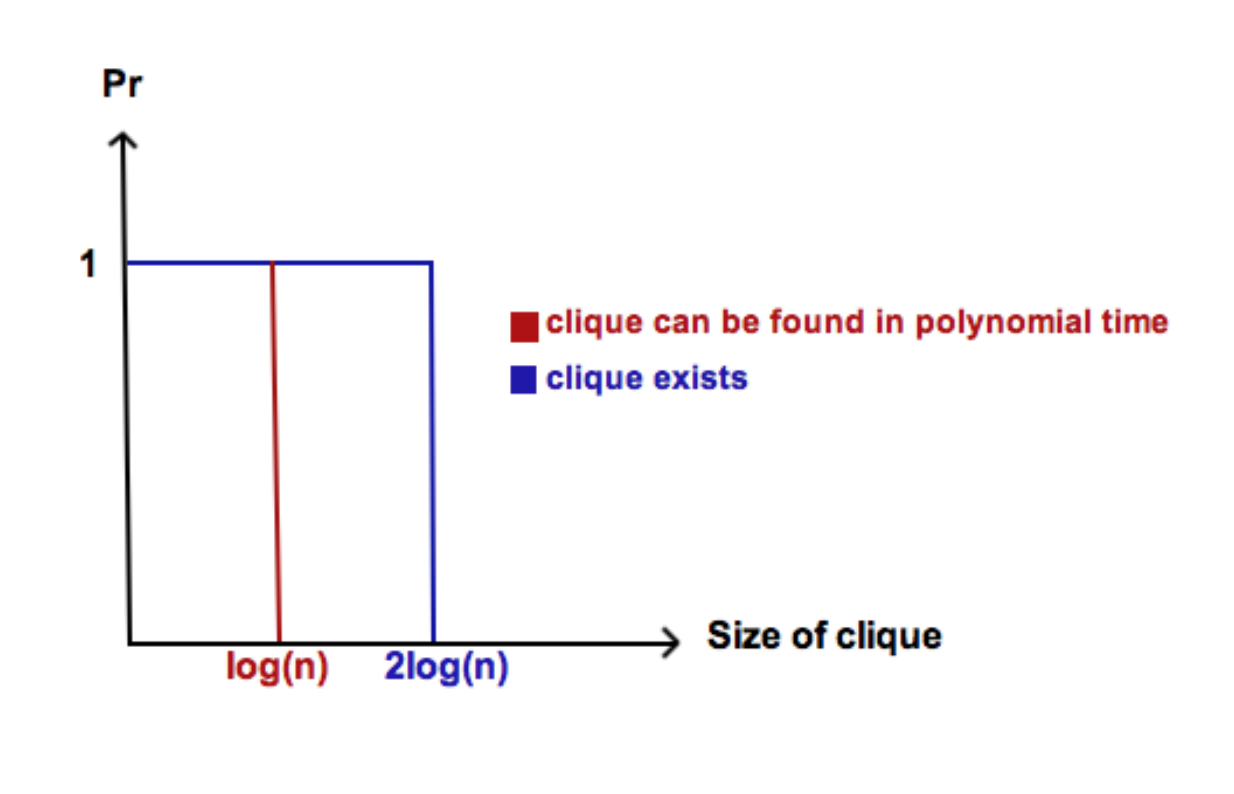
\includegraphics[width=\textwidth]{conclusion}
\end{figure}

\section{References}
A large portion of the second moment method used for the lower bound proof of
the typical size of the largest clique and the above figure are referenced
\href{https://theory.epfl.ch/courses/topicstcs/Lecture1.pdf}{here}.

\end{document}

